\documentclass[a4paper, titlepage]{article}

\usepackage{graphicx}
\usepackage{color}
\usepackage[colorlinks=true]{hyperref}
\usepackage{graphicx}

\begin{document}
	\title{Introduction to git\\ \large An initiative for 1BAinf}
	\date{\today}

	\author{Stijn Rosaer - stijn.rosaer@student.uantwerpen.be\\
	Andrei Bondarenko - andrei.bondarenko@student.uantwerpen.be\\
		Igor Schittekat - igor.schittekat@student.uantwerpen.be\\
	Joey De Pauw - joey.depauw@student.uantwerpen.be\\
	Senne Rosaer - senne.rosaer@student.uantwerpen.be\\
	Toon Meynen - toon.meynen@student.uantwerpen.be
	}
	\maketitle
	
	\tableofcontents
	\section{Intro}
		Github is een versiebeheersysteem waar software geplaatst kan worden. Dit houd in dat men code hier kan plaatsen, updaten, downloaden en terug gaan naar een voorgaande versie. Ook is dit gemakkelijk wanneer men met verschillende personen tezamen werkt aan dezelfde code. We willen zo een overzicht behouden en op een wel bepaald moment elks aan code kunnen werken, zonder dat de code van de ander op dat moment beinvloed wordt.
	

	\pagebreak
	
	\section{How to use git}
		\subsection{Starting with Github}
			\begin{enumerate}
				\item Om github te gebruiken moeten we eerst een account aanmaken. Ga hiervoor naar \href{https://github.com/}{\textit{github.com}} en cre\"eer een account.\\	
				Gebruik zeker je UA-mailadres (voornaam.achternaam@student.uantwerpen.be), je kan namelijk als student gratis private repositories aanmaken. \footnote{Het is ook mogelijk om later je studenten account te linken en alsnog de voordelen te krijgen.}
				\item Voor het aanvragen van je github student developer pack, moet je naar  \href{https://education.github.com/pack}{\textit{education.github.com/pack}} gaan en deze hier aanvragen. Dit kan wat tijd vragen, maar dit hebben we niet nodig om verder te kunnen.
			\end{enumerate}
		\subsection{Github in terminal}
			\begin{enumerate}
				\item Een bestaande github repository downloaden:\\ \textit{git clone [repository url]}
				\item Maak van de huidige map een git repository:\\ \textit{git init [project name]}.
				\item Controleer de status van je git repository:\\ \textit{git status}.
				\item Voeg een of meerdere files toe die je op git wilt bewaren:\\ \textit{git add [filenames]}
				\item Voeg de items toe aan je locale versiebeheer:\\ \textit{git commit -m [bericht met een korte omschrijving van wat je gedaan hebt tussen ""]}
				\item Om dit online te zetten op github en te delen met andere is eerst een repository nodig op github
				\begin{enumerate}
					\item maak een repository aan:\\ 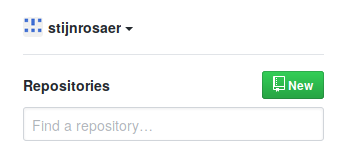
\includegraphics[scale=0.3]{img/maakrepo}\\ vul de nodige gegevens in\\ 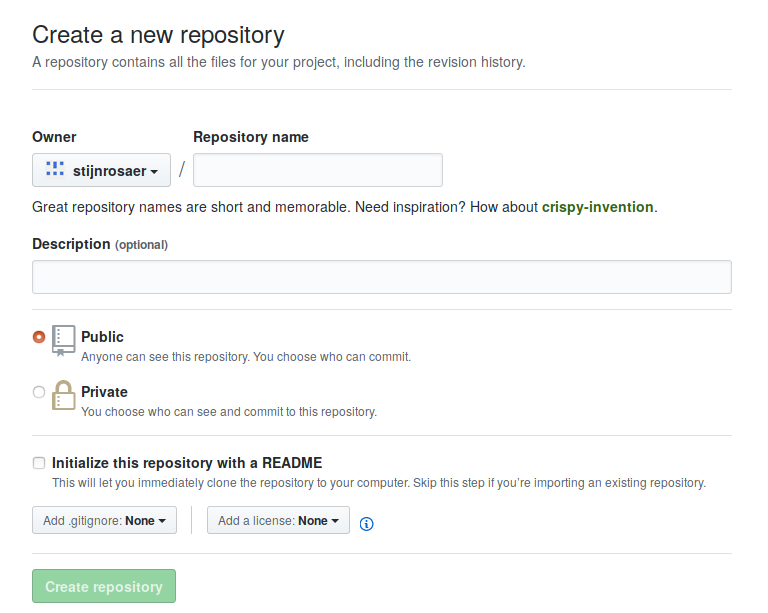
\includegraphics[scale=0.2]{img/maakrepo2}
					\item Voeg je ofline repository toe aan github:\\ \textit{git remote add origin [url van je github repository]}.
				\end{enumerate}
				
				\item Voeg hetgeen je op je pc hebt staan toe op github:\\ git push -u origin master
				
				\item Download de wijzigingen op github:\\ \textit{git pull}
			\end{enumerate}
			
			Een samenvatting en extra features kan je vinden op:\\ \href{https://services.github.com/on-demand/downloads/github-git-cheat-sheet.pdf}{\textit{https://services.github.com/on-demand/downloads/github-git-cheat-sheet.pdf}}
		
		\subsection{Github in PyCharm/CLion}
		\begin{enumerate}
			\item in terminal:\\ \textit{git clone [repository url]}
			\item Maak nu een nieuw project met de map die je juist gecloned hebt aan en klik op JA, dat je de bestanden wilt vervangen
			
			\item Gebruik de blauwe pijl om wijzigingen op te halen en de groene om er zelf door te voeren\\ 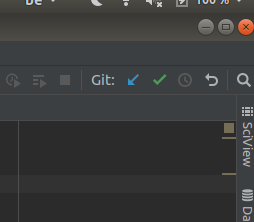
\includegraphics[scale=0.3]{img/pushpull}
			
			\item Voor het toevoegen moet je nog een message geven en zeker niet vergeten om commit en push te kiezen ipv commit
		\end{enumerate}
		
		\subsection{Github rules}
		\begin{enumerate}
			\item push pas wanneer je code compileert, comitten kan je al eerder doen aangezien dit enkel op je computer komt.
			\item 
		\end{enumerate}
		
		\pagebreak
	\section{Exercise}
		\subsection{Maak een repository aan en start een project}
\end{document}

